\documentclass[11pt]{article}
\usepackage[letterpaper,margin=1in]{geometry}
\usepackage{mytex}
\usepackage[colorlinks=true,linkcolor=blue,citecolor=blue]{hyperref}%

\usepackage{bookmark}

\usepackage{newtxtext, kotex}
\usepackage[all,cmtip]{xy}
\usepackage{tikz}
\usepackage{pgfplots}
\usepackage{caption}


\usepackage{fancyhdr}
%\fancyhf{} % sets both header and footer to nothing
\renewcommand{\headrulewidth}{0pt}


\usepackage[textwidth=1in,textsize=small,colorinlistoftodos]{todonotes} % todo 노트

\pagestyle{fancy}
\lhead{Myungsin Cho}
\chead{}
\rhead{}
%\rfoot{\date}

%Bibliography line spacing
% ADD THE FOLLOWING COUPLE LINES INTO YOUR PREAMBLE
\let\OLDthebibliography\thebibliography
\renewcommand\thebibliography[1]{
  \OLDthebibliography{#1}
  \setlength{\parskip}{0pt}
  \setlength{\itemsep}{0pt plus 0.3ex}
}

% section 폰트 바꿔주는거
\usepackage{titlesec}
\titleformat{\section}{\normalfont\large\center}{\thesection}{.5em}{}
\titleformat{\subsection}[runin]{\normalfont\bfseries}{\thesubsection}{.5em}{}

\newcommand{\yourname}{Myungsin Cho}

\newcommand{\univ}{Indiana University}

\newcommand\quelle[1]{{%
      \unskip\nobreak\hfil\penalty50
      \hskip2em\hbox{}\nobreak\hfil #1%
      \parfillskip=0pt \finalhyphendemerits=0 \par}}
      

\usepackage{amsmath,amsfonts,amssymb,mathrsfs}
\usepackage{amsthm,thmtools}
\newtheorem{theorem}{Theorem}
\newtheorem{proposition}{Proposition}
\newtheorem{lemma}{Lemma}
\newtheorem{corollary}[theorem]{Corollary}
\newtheorem*{goal}{Goal}

\let\overto\xrightarrow

\begin{document}
\begin{center}\LARGE{Research Statement}
\end{center}
Algebraic topology began as a way to use algebraic methods to study and classify spaces, but over time it has become central to the interaction between algebra and topology in modern mathematics.
My research investigates how techniques from algebraic topology can clarify the structure of algebraic systems such as number fields and equivariant commutative rings.
For example, my thesis work on extending Tate-Poitou duality in algebraic K-theory to the 2-primary case illustrates how stable homotopy theory connects with arithmetic phenomena.
More broadly, I explore the interplay of stable homotopy theory with algebraic K-theory, equivariant algebra, and combinatorics, aiming to identify precise correspondences between different mathematical descriptions and to develop new tools for studying algebraic invariants and equivariant objects.

\section{Current research and direction}

My current research program is centered around several interconnected projects that explore fundamental structures and relationships in {\it stable homotopy theory}, {\it algebraic K-theory}, and {\it equivariant algebra}, often drawing connections to number theory and combinatorics.


In topology, K-theory studies vector bundles over spaces--families of vector spaces varying continuously with the points of a space. 
Classical examples include the M\"obius band (a non-trivial bundle) and the cylinder (a trivial one) which serve as basic illustrations of different types of vector bundles over a circle:
\vspace{-1.5em} 
\begin{center}
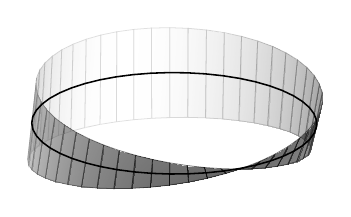
\begin{tikzpicture}[scale=0.7]
\begin{axis}[
    hide axis,
    zmin=-1, zmax=1,
    view={70}{30}
]
\addplot3 [
    surf, shader=faceted interp,
    opacity=0.6,
    point meta=x,
    colormap = {whiteblack}{color(0cm)  = (white);color(1cm) = (black)},
    samples=50,
    samples y=2,
    z buffer=sort,
    domain=0:360,
    y domain=-0.5:0.5
] (
    {(1+0.1*y*cos(x/2))*cos(x)},
    {(1+0.1*y*cos(x/2))*sin(x)},
    {1*y*sin(x/2)});

\addplot3 [
    samples=50,
    domain=-110:250, % The domain needs to be adjusted manually, depending on the camera angle, unfortunately
    samples y=0,
    thick
] (
    {cos(x)},
    {sin(x)},
    {0});
\end{axis}
\end{tikzpicture}
\hspace{2em}
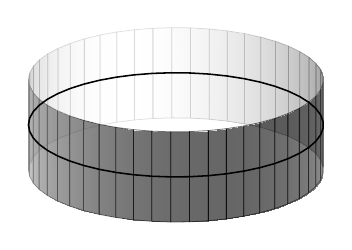
\begin{tikzpicture}[scale=0.7]
\begin{axis}[
    hide axis,
    zmin=-1, zmax=1,
    view={70}{30}
]
\addplot3 [
    surf, shader=faceted interp,
    opacity=0.6,
    point meta=x,
    colormap = {whiteblack}{color(0cm)  = (white);color(1cm) = (black)},
    samples=50,
    samples y=2,
    z buffer=sort,
    domain=0:360,
    y domain=-0.5:0.5
] (
    {cos(x)},
    {sin(x)},
    {y});

\addplot3 [
    samples=50,
    domain=-110:250, % The domain needs to be adjusted manually, depending on the camera angle, unfortunately
    samples y=0,
    thick
] (
    {cos(x)},
    {sin(x)},
    {0});
\end{axis}
\end{tikzpicture}
\\[-1em] % reduce vertical space
\parbox{6cm}{\centering \small M\"obius band over a circle}
\hspace{0em}
\parbox{6cm}{\centering \small Cylinder over a circle}
\end{center}

This perspective produces subtle invariants of spaces and has interactions with many areas of mathematics, from number theory and algebraic geometry to geometric and differential topology. 
In what follows, I describe how my work builds on these ideas, beginning with the interaction between algebraic K-theory and arithmetic duality.

\subsection{Algebraic K-theory and Arithmetic Duality}
My dissertation work explores connections between algebraic K-theory, number theory, and topology, focusing on fundamental questions about the structure of rings of integers in number fields and related objects. {\it Algebraic K-theory} is a powerful invariant that captures both algebraic and geometric information, playing a central role in arithmetic geometry. A fundamental duality algebraic number theory is {\it arithmetic Tate-Poitou duality}, which describes profound relationships between the cohomology groups of number rings and their completions. Motivated by the intricate relationships described by fundamental arithmetic dualities like Tate-Poitou duality, exploring their K-theoretic analogues has become an important direction of investigation.

My work establishes a crucial step towards this goal by proving {\it K-theoretic Tate-Poitou duality at prime 2}. This theorem provides a homotopical refinement of the classical arithmetic duality, revealing structural relationships within the {\it $K(1)$-localized algebraic K-theory} of a number ring and its completions.
\begin{theorem}[\cite{Cho}]
Let $F$ be a number field.
There is a canonical weak equivalence between  the {\it homotopy fiber of the completion map} $\ka$ in $K(1)$-local algebraic K-theory:
\[\ka: L_{K(1)}K(\calO_F[\tfrac{1}{2}]) \longrightarrow \prod_{\nu \mid 2} L_{K(1)}K(F_\nu^\w)\]
and the $\bZ_2$-Anderson dual of the algebraic $K$-theory of $\calO_F[\tfrac{1}{2}]$:
 \begin{equation}\label{fib}
 \Fib(\ka) \simeq \SI^{-1} I_{\bZ_2} L_{K(1)}K(\calO_F[\tfrac{1}{2}]).
\end{equation}
\end{theorem}

A significant application and consequence of this main duality theorem is a new insight into the algebraic K-theory of the {\it sphere spectrum} ($\bS$).
Using the case $F=\bQ$ together with {\it trace methods}, one obtains the following result.
\begin{corollary}[\cite{Cho}]
Let $\ta_\bS: K(\bS)_2^\w \to TC(\bS)_2^\w$ be the $2$-completed cyclotomic trace map for the sphere spectrum.
After taking connective covers, the homotopy fiber $\Fib(\ta_\bS)$ is canonically weakly equivalent to the $\bZ_2$-Anderson dual of $L_{K(1)}K(\bZ)$:
\[\Fib(\ta\bS)[0,\infty) \simeq \Sigma^{-1} I{\bZ_2}\, L_{K(1)}K(\bZ)[0,\infty).\]
\end{corollary}
This result makes explicit calculations in $K(\bS)_2^\w$ possible, and shows how the homological behavior of the integers enters stable homotopy theory through algebraic K-theory.

It also extends foundational results of Blumberg, Mandell, and Yuan \cite{MR4121155,BMY}, who proved the duality at odd primes and conjectured its validity for $p=2$. The prime $2$ case presents distinctive challenges because of the essential role of real embeddings of number fields, which fundamentally change the behavior of related invariants and require new technical methods not needed in the odd prime case.

Furthermore, the homotopy fiber of the completion map $\Fib(\ka)$ that appears in (\ref{fib}) is known to be related to objects studied in other areas, including the {\it $p$-adic Langlands correspondence} \cite{MR2905536} and {\it compactly supported K-theory} \cite{MR3211458}. 
By giving a precise description of $\Fib(\ka)$, my work sets the stage for examining how it interacts with related structures with these structures.

This research develops new methods in 2-primary algebraic K-theory that clarify the structure of number rings and yield concrete tools for studying central objects such as the sphere spectrum.
The K-theoretic Tate-Poitou duality established here has numerous potential implications and suggests several directions for future investigation in more general settings.

\subsection{Real algebraic K-theory and homological trace methods}
Another ongoing project focuses on {\it real algebraic K-theory}, introduced by Hesselholt and Madsen \cite{HMreal}, which assigns genuine $C_2$-equivariant spectra to rings with an {\it anti-involution}.
It refines and unifies classical algebraic K-theory, Hermitian K-theory, and L-theory by incorporating this additional symmetry.
Through this perspective, one can study rings with anti-involution in a way that connects naturally to questions in topology and geometry, and recent work has shown that computational methods from equivariant homotopy theory are particularly effective in this setting.

In collaboration with Teena Gerhardt, Liam Keenan, Juan Moreno, and J.D. Quigley, we are extending {\it homological trace methods} due to Bruner and Rognes \cite{MR2153113} to the $C_2$-equivariant setting. 
Our work develops a new spectral sequence based on $RO(C_2)$-graded homology, designed to provide computational access to invariants in real algebraic K-theory. 
\begin{theorem}[Gerhardt--C.--Keenan--Moreno--Quigley]
 For a $C_2$-equivariant $\ef$-ring spectrum $R$ with twisted $\bT$-action, there is a natural $\aA_\ast^{C_2}$-comodule algebra spectral sequence of Mackey functors:
 \[E^2_{\ast,\star} = H^{-\ast}(B_{C_2}\bT; H \ul{\bF_2}_\star (R)) \Rightarrow H\ul{\bF_2}_\star^c (R^{h_{C_2}\bT})\]
\end{theorem}
This refinement of classical trace methods to the $C_2$-equivariant setting is motivated by the need for concrete computational tools in real algebraic K-theory. It provides a method for studying equivariant invariants and enables approximations for important spectra, most notably the {\it real bordism spectrum} ($MU_\bR$).

Recent progress in real algebraic K-theory has come through the development of {\it real trace methods}, computational techniques grounded in equivariant stable homotopy theory.
These have produced $C_2$-equivariant analogues of classical tools, including {\it real topological Hochschild homology} \cite{Dotto} and {\it real topological cyclic homology} \cite{Hogenhaven}.
Our extension of homological trace methods builds directly on this line of work.

The long-term goal of this project is to use these methods to analyze the real algebraic K-theory of important spectra such as $MU_\bR$ and the {\it real Brown–Peterson spectrum} ($BP_\bR$).
In particular, we aim to establish a {\it real analogue of the Segal conjecture} for these spectra, which would serve as the essential step toward their approximation.
Achieving such an analogue would furnish concrete computational tools and clarify the relationship between real algebraic K-theory and its trace method approximations.


\subsection{Equivariant algebras and homotopical combinatorics}
My research in {\it equivariant algebra} focuses on {\it transfer systems} \cite{MR4244201}, which encode the combinatorial structure behind algebraic operations arising from equivariant stable homotopy theory.
A transfer system is essentially a way of selecting a subset of possible ``{\it transfer}'' operations between subgroups, subject to natural coherence conditions such as compatibility with conjugation and restriction.
They provide the combinatorial input for understanding algebraic structures (e.g., {\it Tambara functors}) that arise in equivariant stable homotopy theory.

Tambara functors \cite{MR1209937} arise as the $\pi_0$ of commutative $G$-ring spectra in genuine equivariant stable homotopy theory, and admit natural variations such as {\it incomplete} and {\it bi-incomplete} Tambara functors \cite{MR3773736,MR4327103}.
The structure of these functors--particularly the presence or absence of certain additive (transfers) and multiplicative (norms) operations--is precisely determined by the data of the associated transfer systems, subject to natural coherence conditions \cite{MR4696086}, often formulated as the requirement that the additive and multiplicative transfer systems form a compatible pair.
In this way, transfer systems provide the link between combinatorial data and the $N_\infty$-operad which parametrizes the admissible operations on commutative $G$-ring spectra.

In collaboration with David Chan, David Mehrle, Pablo Sanchez Ocal, Angelica Osorno, Ben Szczesny, and Paula Verdugo, our work aims to establish an equivalence between two descriptions of the structures governing incomplete Tambara functors. 
One is a combinatorial description using compatible pairs of transfer systems, and the other is a homotopical description using {\it pairing of operads} \cite{MR2544392}. Our team has proved one direction of this equivalence, and a partial result toward the converse.
\begin{theorem}[Chan--C.--Mehrle--Sanchez Ocal--Osorno--Szczesny--Verdugo]
An action of one $N_\infty$-operad on another implies that their associated transfer systems form a compatible pair.
If a compatible pair of transfer systems has a complete additive component, then there exists a pairing of $N_\infty$-operads that realizes it.
\end{theorem}
A primary goal of our ongoing work is to prove the converse in full generality--that any compatible pair of transfer systems can be realized as an $N_\infty$-operad action. Achieving this equivalence would provide a unified framework for understanding the structures governing incomplete Tambara functors, bridging combinatorial and operadic perspectives.


\section{Future research direction}

My future research direction build directly on my current work, extending results on duality phenomena in algebraic K-theory and pursuing further developments in equivariant algebra.
I am also interested in exploring connection to complex geometry, where tools from algebraic K-theory and equivariant methods may reveal new interactions.
In addition to these research programs, I plan to create opportunities for accessible projects that emphasize concrete computations and examples, particularly in areas such as homotopical combinatorics and topological data analysis.
These topics are well suited for undergraduate involvement and provide natural entry points into algebraic topology and I see engaging students in such projects as an essential part of advancing the field and training the next generation of researchers.

\subsection*{Duality and Symmetry in Algebraic K-theory}
Building on my work on K-theoretic Tate-Poitou duality, I plan to extend these ideas in several directions: higher-dimensional analogues, chromatic refinements, and new formulations in the real algebraic K-theory setting.

One natural line of investigation is the study of higher dimensional versions of the K-theoretic duality.
While progress has been made for odd primes \cite{Braunling}, the case at prime 2 remains open.
Building on the methods I developed to address the unique challenges at prime 2, I aim to extend these higher-dimensional results to include this case.

Another direction concerns higher chromatic height in stable homotopy theory.
Initial results \cite{HRW} suggest that the connective Adams' summand spectra $l$ exhibit behavior reminiscent of local rings in arithmetic geometry.
This raises the possibility of a chromatic analogue of arithmetic duality, and my goal is to establish a K-theoretic duality in this setting.

Beyond these extensions, I am also focused on real algebraic K-theory.
An ultimate goal is to develop a {\it real Thomason spectral sequence}, providing a systematic tool for its computation.
Constructing such a spectral sequence requires a genuine equivariant framework for \'etale cohomology of equivariant commutative rings, and my plan is to begin by building this language and then adapting classical descent spectral sequence constructions to the real equivariant setting.
This project has the potential to open a new computational approach to real algebraic K-theory, paralleling the role of Thomason’s spectral sequence in the classical setting.


\subsection*{Foundations for Equivariant Algebra}
While advanced structures like Tambara functors are powerful tools in equivariant stable homotopy theory, many fundamental algebraic notions that are standard for classical rings have not yet been systematically developed in this setting.

A natural entry point is the study of commutative $G$-rings, a simpler type of equivariant algebraic object that Tambara functors generalize.
Even here, basic concepts such as algebraic extensions and algebraic closures present subtle challenges.
Investigating these questions for $G$-rings offers a concrete starting point that is accessible even to undergraduate students, while also providing insight and methods that can inform the more general theory of Tambara functors.
Beginning with these more manageable cases allows one to build intuition and techniques before addressing the full complexity of Tambara functor structures.

My goal is to establish such fundamental concepts and structures within the equivariant setting.
This foundational work is a necessary step toward developing an algebraic geometry of Tambara functors, playing a role analogous to commutative algebra in classical algebraic geometry.


\subsection*{Analytic Stacks and Hyperbolicity}
Another direction of my research concerns the study of {\it hyperbolicity} in the setting of stacks.
In complex geometry, notions of hyperbolicity--such as those of {\it Brody} or {\it Kobayashi}--capture rigidity phenomena and asymptotic constraints on holomorphic maps.
Work of Borghesi and Tomassini \cite{MR3673667} has extended these ideas to {\it stacks} and {\it simplicial presheaves}, showing that hyperbolicity can be meaningfully formulated and studied beyond the classical setting of complex manifolds.

Building on their framework, my collaborator Geonhee Cho and I aim to extend the theory further to higher stacks and to incorporate additional notions of hyperbolicity.
An important part of this program is to construct and analyze concrete examples that illustrate how these generalized notions behave in practice.
I am particularly interested in clarifying how hyperbolicity can be formulated and detected in derived settings, and in understanding what kinds of rigidity phenomena or structural constraints arise in relation to the homotopy theory of stacks

This project not only expands the reach of hyperbolicity beyond classical complex spaces but also connects it to modern homotopical and stack-theoretic methods. By pursuing these extensions, this approach has the potential to reveal new phenomena related to automorphism groups, curvature, and symmetry in geometric objects that lie beyond the traditional scope of complex geometry.


\subsection*{Undergraduate Research Directions}
Several aspect of my work also give rise to problems and projects that are accessible at an undergraduate level yet remain connected to broader research questions.
Two areas in particular--transfer systems and topological data analysis--offer tractable problems that can both engage undergraduate and contribute to the development of my research programs.

One direction is the study of {\it transfer systems} from a combinatorial perspective.
Transfer systems are defined directly in terms of subgroup lattices, making them elementary to state while still encoding the algebraic constraints that govern equivariant operations.
Questions such as counting finite posets associated with transfer systems are approachable for students, yet they also inform the broader theory of $N_\infty$-operads and Tambara functors by clarifying how combinatorial constraints control admissible algebraic operations.
This line of investigation illustrates how even elementary combinatorics can feed directly into ongoing developments in equivariant algebra.

Another area is {\it topological data analysis} (TDA), which applies algebraic topology to study the structure of high-dimensional data set.
Methods such as {\it persistent homology} can be introduced in a straightforward and visual way, but they also open into deeper questions about stability, functoriality, and even the role of cohomology operations.
These connections are currently an active area of research, and concrete case studies in TDA provide a natural testing ground for exploring how homotopical invariants can yield new insights into the geometry of data.

In this way, projects in combinatorics and TDA serve not only as entry points for undergraduate participation but also as stepping stones toward more advanced problems aligned with my core research agenda.


\section{Conclusion}
Across these projects, a unifying theme of my research is the use of duality, symmetry, and equivariant structures to connect algebra, topology, and geometry.
From establishing K-theoretic Tate-Poitou duality at prime 2, to developing foundations for equivariant commutative algebra, to extending notions of hyperbolicity to derived stacks, my works focus how homotopical methods can clarify and connect seemingly disparate parts of mathematics.

Looking ahead, my long term goal is to build a coherent research program where these methods not only advance our understanding of (real) algebraic K-theory and equivariant algebra, but also provide computational tools and conceptual frameworks that other can build on.
Equally important to me is ensuring that parts of this program remain accessible at multiple levels, including problems suitable for undergraduate research.
In this way, my research combines technical development with opportunities for broad participation.

\bibliography{RS_bib}
\bibliographystyle{alphaurl}

\end{document}